\chapter{Theorie}
\label{cha:Theorie}

\section{Röntgenstrahlung}

Röntgenstrahlen sind elektromagnetische Wellen, welche eine Wellenlänge zwischen $\qty{5}{\pico\metre}$ und $\qty{10}{\nano\metre}$ aufweisen.
Dies entspricht Energien von
\begin{equation*}
    E_{\lambda} = \frac{hc}{\lambda} \Rightarrow \qtyrange{120}{250000}{\electronvolt},
\end{equation*}
wobei $h$ das Plancksche Wirkungsquantum, $c$ die Lichtgeschwindigkeit und $\lambda$ die Wellenlänge ist. Auf dem Wellenlängenspektrum ist Röntgenstrahlung
oberhalb des ultravioletten Bereichs einzuordnen. Da es sich bei Röntgenstrahlung um ionisierende Strahlung handelt, ist eine direkte Exposition mit lebenden
Organismen möglichst zu vermeiden. Neben nützlichen Anwendungen im medizinischen Sektor, wird Röntgenstrahlung auch vorallem in der Spektroskopie verwendet,
um Multischichtsysteme zu untersuchen, bei denen die Schichten nur wenige Nanometer breit sind.

\subsection{Erzeugung von Röntgenstrahlung}
Röntgenstrahlung wird in Röntgenröhren erzeugt. Diese evakuierten Röhren bestehen aus einer Kathode und einer Anode, wobei das Anodenmaterial aus einem Metall besteht. 
Es wird an Kathode und Anode eine Spannung angelegt, woraufhin sich Elektronen aus der Kathode lösen und durch ein Feld zur Anode hin beschleunigt werden. Die 
beschleunigten Elektronen treffen schließlich auf das Anodenmaterial, wo sie stark abgebremst werden. Hier treten zwei verschiedene Effekte auf, welche beide
zum resultierenden Strahlungsspektrum beitragen.\\
Durch ein Abbremsen an dem Coulombfeld der Anodenatome, entsteht ein kontinuierliches Bremsspektrum. Es entsteht zudem ein diskretes Energiespektrum dadurch,
dass Elektronen der Anodenatome durch Stöße mit den beschleunigten Elektronen aus ihrer Schale befreit werden. Hierbei fällt anschließend ein Elektron aus einem
höheren Energieniveau in das darunter hinab, wobei die Energiedifferenz durch Photonen davongetragen wird. Diese befinden sich ebenfalls im Röntgenspektrum.
Diese charakteristischen Linien im Röntgenspektrum sind abhängig vom Anodenmaterial und können nur Werte annehmen, welche mit den Energiedifferenzen der Energieniveaus
übereinstimmen. Ein Beispiel eines Röntgenspektrums ist in \autoref{fig:roentgenspektrum} dargestellt.
\begin{figure}
    \centering
    \includegraphics[width = 0.7\textwidth]{bilder/Röntgenspektrum.png}
    \caption{Ein beispielhaftes Röntgenspektrum \cite{Uni_Goett}.}
    \label{fig:roentgenspektrum}
\end{figure}

\subsection{Röntgenstrahlung an Grenzflächen}

Trifft elektromagnetische Strahlung auf Grenzflächen, wird ein Teil der Intensität reflektiert, während der andere gebrochen wird. Die Ausbreitungsrichtung der Brechung,
sowie der Reflexion lasen sich aus dem Snelliusschen Brechungsgesetz \autoref{eq:Snell_Brech}(für den gebrochenen Strahl), beziehunsgweise dem Reflexionsgesetz \autoref{eq:Reflexionsgesetz}(für den reflektierten Strahl) berechnet werden:
\begin{align}
\label{eq:Snell_Brech}
    \eta_1 \sin{\theta_1} &= \eta_2 \sin{\theta_2}\\
\label{eq:Reflexionsgesetz}
    \theta_1 &= \theta_2.
\end{align}
$\theta_1$ ist der Winkel des einfallenenden (beziehunsgweise ausfallenden $\theta_2$) zu dem Einfallslot, welches senkrecht auf dem Material steht. $\eta_1$ ist der komplexe Brechungsindex des Materials aus dem der Strahl kam und
$\eta_2$ der komplexe Brechungsindex des Materials in das der Strahl reingebrochen wird.\\
Der komplexe Brechungsindex ist materialspezifisch und kann für sehr kurzwellige Wellen wie die Röntgenstrahlung über
\begin{equation}
    \label{eq:Brechungsindex}
    \eta = 1-\delta+iK
\end{equation}
bestimmt werden. $\delta$ ist ein Korrekturfaktor und stark abhängig von der Wellenlänge, Ordnungszahl und Dichte des Materials. Allgemein liegt er für das Röntgenspektrum zwischen $\qty{10e-9}{}$ und $\qty{10e-5}{}$.
$K$ ist die Absorption des Mediums und ebenfalls materialabhängig. Die Größen lassen sich durch
\begin{align}
    \delta &= \frac{\lambda^2}{2\pi}r_e\rho\\
    K &= \frac{\lambda}{4\pi}\mu(r)
\end{align}
berechnen. Hier steht $\lambda$ erneut für die Wellenlänge des Strahls, $\rho$ für die Dichte des Materials, $r_e$ für den Elektronenradius und $\mu(r)$ ist der lineare Absorptionskoeffizient.\\
Die Intensitätsanteile des reflektierten und transmittierten Strahlteile lassen sich durch die Fresnelformeln bestimmen. Diese sind gegeben durch:
\begin{align}
    r &= \frac{\eta_1 \sin{\theta_1} - \eta_2 \sin{\theta_2}}{\eta_1 \sin{\theta_1} + \eta_2 \sin{\theta_2}},\\
    t &= \frac{2\eta_1 \sin{\theta_1}}{\eta_1 \sin{\theta_1} + \eta_2 \sin{\theta_2}}.
\end{align}
Wenn ein Röntgenstrahl von Luft ($\eta = 1$) in ein optisch dünneres Medium tritt ($\eta_2 < \eta_1$), dann tritt unter einem Winkel der Totalreflexion
keine Brechung des Strahls mehr auf. Dieser kritische Winkel lässt sich als
\begin{equation}
    \label{eqn:theta_total}
    \theta_c \approx \sqrt{2\delta} = \lambda \sqrt{\frac{r_e \rho}{\pi}}
\end{equation}
nähern. 
Die Reflektivität (beziehunsgweise Transmitivität) lässt sich durch das Betragsquadrat $R = |r|^2$ ($T= |t|^2$) bestimmen. Falls $\theta_1 > 3 \theta_c$,
lässt sich die Reflektivität nähern mit:
\begin{equation}
    R = \left(\frac{\theta_c}{2\theta_1}\right)^4.
\end{equation}

\section{Multischichtsysteme}
Wenn elektromagnetische Strahlung auf ein System trifft, das aus vielen verschiedenen geschichteten Materialien besteht, dann wird dieser Strahl an jeder Grenzschicht transmittierten und reflektiert. 
Bei jedem Grenzübergang wird der Anteil der transmittierten Strahlung geringer. Zudem interferieren die reflektierten Strahlen mit den transmittierten der vorherigen Schichten. Resulierend bilden sich
abhängig von Einfallswinkel Oszillationen im Intensitätsspektrum der reflektierten Strahlung. Diese Oszillationen werden als Kiessig Oszillationen bezeichnet und sind in \autoref{fig:Oszillationen} dargestellt.
\begin{figure}
    \centering
    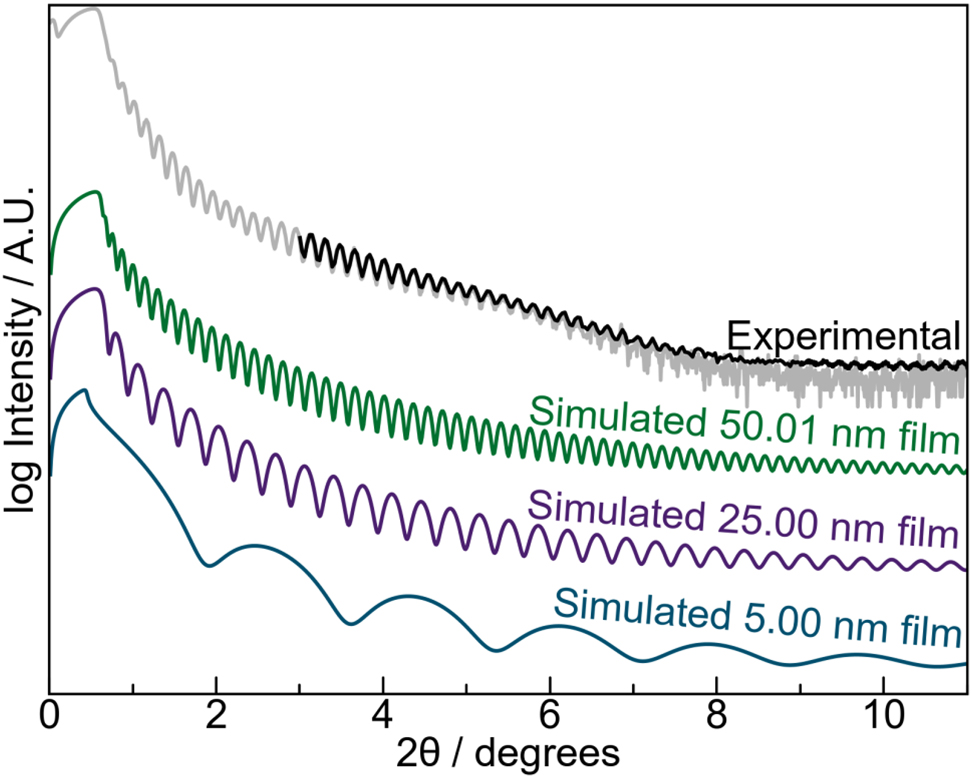
\includegraphics[width = 0.7\textwidth]{bilder/Oszillationen.jpg}
    \caption{schematische Darstellung der Kiessig Oszillationen (farbig) und eine experimentelle Messung dieser Oszillationen (schwarz)\cite{Kiessig}.}
    \label{fig:Oszillationen}
\end{figure}
Da diese Interferenzen und somit Oszillationen stark von der in den Schichten zurückgelegten Strecke abhängen, lassen sich die Schichdicken anhand der lokalen Maxima der Oszillation berechnen:
\begin{equation}
    \label{eqn:Schichtdicke}
    d = \frac{\lambda}{2\Delta \theta}.
\end{equation}
Hierbei ist $\lambda$ die Wellenlänge des Röntgenstrahls und $\Delta \theta$ der Abstand zweier Extrema.\\
Unter der Annahme, dass die letzte Schicht eines Multischichtsystems unendlich dick ist, hiernach also keine Reflexion mehr auftritt, kann der Parratt-Algorithmus verwendet werden um die Gesamtreflektivität
zu bestimmen. Dieser Algorithmus verwendet eine Rekursionsformel:
\begin{equation}
    X_j = \frac{R_j}{T_j} = \exp{(-2ik_z  z_j)}\frac{r_{j,j+1}+X_{j+1}\exp{(2ik_{z,j+1}z_j)}}{1+r_{j,j+1}X_{j+1}\exp{(2ik_{z,j+1}z_j)}}.
\end{equation}
Hierbei ist $z_j$ die jeweilige Grenzschicht, $r_{j,j+1}$ der Reflektionskoeffizient nach Fresnel und $k_{z,j}$ die $z$-Komponente der jeweiligen Schicht mit $k_{z,j} = \sqrt{\eta_j^2 - \cos^2{\theta_1}}$. Durch
die Annahme, dass die letzte Schicht unendlich dick sein soll, ergibt sich $X_{N+1} =0$ als Startwert für den Parratt-Algorithmus.\\
Der Parratt-Algorithmus nimmt an, dass alle Oberfläche perfekt glatt und gerade ist, sodass die Schichtdicke ein konstanter Wert ist. In einem reellen System ist dich durch Verbiegungen und Schäden am Material allerdings
nicht der Fall, daher muss der Paratt-Algorithmus um eine gewisse Rauigkeit korrigiert werden. Für diee Rauigkeit wird angenommen, dass die Schichtdicken größer sind als die Unebenheiten, wodurch sie mit 
einer root-mean-square-Funktion angenähert werden kann:
\begin{equation}
    \label{eqn:rauigkeit}
    \sigma_j^2 = \int (z-z_j)^2P_j(z)dz
\end{equation}
$P_j(z)$ bezeichnet hier die Wahrscheinlichkeit, dass die j-te Grenzschicht im Intervall [$z_j+z$, $z_j+z+dz$] befindet, wobei $z_j$ die exakte theoretische Position dieser Grenzschicht ist. Als Wahrscheinlichkeitsverteilung
wird eine Normalverteilung mit der Breite $\sigma_j$ gewählt. Die Fresnel-koeffizienten werden dementsprechend um die eingeführte Rauigkeit ergänzt:
\begin{align}
    \label{eqn:fresnel_ref}
    \tilde{r}_{j,j+1} &= r_{j_j+1} \exp{(-2k_{z,j}k_{z,j+1}\sigma^2)},\\
    \tilde{t}_{j,j+1} &=  t_{j_j+1} \exp{(\frac{1}{2}(k_{z,j}-k_{z,j+1})^2\sigma^2)}.
\end{align}
Diese korrigierten Koeffizienten werden im Parratt-Algorithmus verwendet.

\section{Korrekturen}
Ab einem gewissen Grenzwinkel $\theta_g$ ist die Strahlbreite größer, als die Projektion der Materialoberfläche auf die Wellenfront des Strahls, wodurch ein Teil der Strahl nicht mehr auf das Material trifft. Hier hat man also
systematische Intensitätsverluste, die ausgeglichen werden. Dies wird durch die Korrektur um einen Geometriefaktor vorgenommen. Der Winkel, ab dem eine Korrektur stattfinden muss ist gegeben durch
\begin{equation}
    \label{eqn:Geometriewinkel}
    \theta_g = \arcsin{(\frac{d_0}{D})},
\end{equation}
wobei $d_0$ die Strahlbreite ist und $D$ die Länge der Materialoberfläche. Der Geometriefaktor um den korrigiert werden soll ergibt sich schließlich als
\begin{empheq}[left={G =\empheqlbrace}]{alignat*=2}
    & \frac{D \sin{\theta_1}}{d_0}                    && \text{für}\ \theta_1 < \theta_g \\
    & 1                && \text{für}\ \theta_1 \geq \theta_g.
\end{empheq}
$D \sin{\theta_1}$ ist die Projektion der Materialoberfläche auf den Strahl.